%==============================================================================
% Tento soubor použijte jako základ
% This file should be used as a base for the thesis
% Autoři / Authors: 2008 Michal Bidlo, 2022 Jaroslav Dytrych, 2025 Petr Veigend
% Kontakt pro dotazy a připomínky: sablona@fit.vutbr.cz
% Contact for questions and comments: sablona@fit.vutbr.cz
%==============================================================================
% kódování: UTF-8 (zmena prikazem iconv, recode nebo cstocs)
% encoding: UTF-8 (you can change it by command iconv, recode or cstocs)
%------------------------------------------------------------------------------
% zpracování / processing: make, make pdf, make clean
%==============================================================================
% Soubory, které je nutné upravit nebo smazat: / Files which have to be edited or deleted:
%   projekt-20-literatura-bibliography.bib - literatura / bibliography
%   projekt-01-kapitoly-chapters.tex - obsah práce / the thesis content
%   projekt-01-kapitoly-chapters-en.tex - obsah práce v angličtině / the thesis content in English
%   projekt-30-prilohy-appendices.tex - přílohy / appendices
%   projekt-30-prilohy-appendices-en.tex - přílohy v angličtině / appendices in English
%==============================================================================

\documentclass[12pt,a4paper]{report}
\usepackage[utf8]{inputenc}
\usepackage[T1]{fontenc}
\usepackage[main=english,czech]{babel}

\usepackage{geometry}
\geometry{margin=2.5cm}
\usepackage{hyperref}
\hypersetup{
  colorlinks=true,
  linkcolor=black,
  urlcolor=blue,
  citecolor=black
}

\usepackage{listings}
\usepackage{caption}
\usepackage{enumitem}
\usepackage{float}
\usepackage{longtable}
\usepackage{array}
\usepackage{booktabs}
\usepackage{url}
\usepackage{titling}
\usepackage{graphicx}

\lstset{
  basicstyle=\ttfamily\small,
  breaklines=true,
  columns=fullflexible,
  frame=single,
  showstringspaces=false
}

\title{FITNESS APPROXIMATION FOR GENETIC PROGRAMMING \\[4pt]
\large APROXIMACE FITNESS PRO GENETICKÉ PROGRAMOVÁNÍ\\[1em]
BACHELOR'S THESIS\\
BAKALÁŘSKÁ PRÁCE}

\author{Stepan Kravchenko}
\date{}

\begin{document}

% --- TITLE PAGE ---
\begin{titlepage}
\begin{flushleft}

\includegraphics[width=0.25\textwidth]{Screenshot 2025-11-06 at 23.24.17}\\[1cm]

{\large \textbf{BRNO UNIVERSITY OF TECHNOLOGY}}\\[0.3cm]
{\large \textbf{VYSOKÉ UČENÍ TECHNICKÉ V BRNĚ}}\\[0.5cm]

{\large \textbf{FACULTY OF INFORMATION TECHNOLOGY}}\\
{\large \textbf{FAKULTA INFORMAČNÍCH TECHNOLOGIÍ}}\\
{\large \textbf{Department of Computer Systems}}\\
{\large \textbf{Ústav počítačových systémů}}\\[1.5cm]

{\LARGE \textbf{FITNESS APPROXIMATION FOR GENETIC PROGRAMMING}}\\[0.4cm]
{\LARGE \textbf{APROXIMACE FITNESS PRO GENETICKÉ PROGRAMOVÁNÍ}}\\[0.5cm]
{\Large \textbf{BACHELOR'S THESIS}}\\
{\Large \textbf{BAKALÁŘSKÁ PRÁCE}}\\[1.5cm]

\begin{tabular}{@{}l r@{}}
\textbf{AUTHOR} & \makebox[10cm][r]{Stepan Kravchenko} \\[0.4cm]
\textbf{AUTOR PRÁCE} & \\[0.4cm]
\textbf{SUPERVISOR} & \makebox[10cm][r]{Ing. Martin Hurta} \\[0.4cm]
\textbf{VEDOUCÍ PRÁCE} & \\[1.5cm]
\end{tabular}

\vspace{0.8cm}
{\large \textbf{BRNO 2026}}

\end{flushleft}
\end{titlepage}

% --- BACHELOR'S THESIS ASSIGNMENT ---
\begin{titlepage}
\begin{flushleft}
\small

\includegraphics[width=0.75\textwidth]{Screenshot 2025-11-07 at 16.59.32}\\[0.8cm]

{\LARGE \textbf{Bachelor's Thesis Assignment}}\\[0.5cm]

{\large \textbf{Institut: Department of Computer Systems (DCSY)}}\\[0.3cm]

\textbf{Student:} Stepan Kravchenko\\
\textbf{Program:} Information Technology\\
\textbf{Title:} Fitness Approximation for Genetic Programming\\
\textbf{Category:} Artificial Intelligence\\
\textbf{Academic year:} 2025/26\\[0.5cm]

\textbf{Assignment:}
\begin{enumerate}[leftmargin=1.2cm]
    \item Study the Genetic Programming (GP) and its possibilities for solving selected tasks.
    \item Study the issue of fitness approximation within evolutionary algorithms.
    \item Write a study on the above topics.
    \item Propose a method for fitness approximation within GP.
    \item Implement the proposed method.
    \item Experimentally verify the proposed method on a selected problem and compare it with the basic variant of GP.
    \item Evaluate the results achieved and discuss the possibilities of further development.
\end{enumerate}

\vspace{0.5cm}
\textbf{Literature:}\\
Koza, J. R. \emph{Genetic programming : On the programming of computers by means of natural selection}. Cambridge : London,: Bradford Book, MIT Press, 1992. Complex adaptive systems. ISBN 0-262-11170-5.\\
Miller, J. F. \emph{Cartesian genetic programming: its status and future}. Genetic programming and evolvable machines. New York: Springer US, 2020, vol. 21, 1-2, p. 129–168. ISSN 1389-2576. Available at: \url{https://doi.org/10.1007/s10710-019-09360-6}.\\
Jin, Y. \emph{A comprehensive survey of fitness approximation in evolutionary computation}. Soft computing (Berlin, Germany). NEW YORK: Springer Nature, 2005, vol. 9, no. 1, p. 3–12. ISSN 1432-7643. Available at: \url{https://doi.org/10.1007/s00500-003-0328-5}.

\vspace{0.5cm}
\textbf{Requirements for granting of credit for semester work:} First four points of the assignment.

\vspace{0.8cm}
\textbf{Supervisor:} Ing. Martin Hurta\\
\textbf{Head of Department:} Sekanina Lukáš, prof. Ing., Ph.D.\\
\textbf{Beginning of work:} 04.11.2025\\
\textbf{Submission deadline:} 13.5.2026\\
\textbf{Approval date:} TBD

\vfill
\end{flushleft}
\end{titlepage}

% --- ROMAN PAGE NUMBERS ---
\pagenumbering{roman}
\setcounter{page}{1}

% --- ABSTRACT ---
\section*{Abstract}
This thesis deals with the approximation of the fitness function in Genetic Programming (GP), which is one of the key components influencing the efficiency and convergence of evolutionary algorithms. The main objective of this work is to reduce the computational cost of the evolutionary process by estimating the fitness values of new individuals based on knowledge obtained from previously evaluated solutions.
The thesis first provides a theoretical overview of genetic programming, including the basic principles of evolution, representation of individuals, and fitness evaluation. It then analyses existing approaches to fitness approximation and discusses their advantages, limitations, and practical use.
In the practical part, a new approximation method is proposed, implemented, and experimentally tested on selected symbolic regression problems. The results demonstrate that the proposed approach can significantly reduce the number of full evaluations while maintaining a comparable level of accuracy. The work concludes with a discussion of achieved results and possible directions for further research.

\section*{Abstrakt}
Tato práce se zabývá aproximací fitness funkce v genetickém programování (GP), které představuje jednu z klíčových součástí evolučních algoritmů ovlivňujících jejich efektivitu a konvergenci. Hlavním cílem práce je snížit výpočetní náročnost evolučního procesu pomocí odhadu hodnot fitness nových jedinců na základě znalostí získaných z již vyhodnocených řešení.
V teoretické části je uveden přehled principů genetického programování, reprezentace jedinců a vyhodnocování jejich kvality. Následně jsou analyzovány existující přístupy k aproximaci fitness, jejich výhody, nevýhody a možnosti praktického využití.
V praktické části je navržena a implementována nová metoda aproximace, která byla experimentálně ověřena na úloze symbolické regrese. Výsledky ukazují, že navržený přístup může výrazně snížit počet úplných vyhodnocení při zachování srovnatelné přesnosti. Práce je zakončena shrnutím dosažených výsledků a návrhem možných směrů dalšího výzkumu.

\section*{Keywords}
Genetic Programming, Fitness Approximation, Evolutionary Algorithms, Symbolic Regression, Python.

\section*{Klíčová slova}
Genetické programování, aproximace fitness, evoluční algoritmy, symbolická regrese, Python.

\newpage
\section*{Rozšířený abstrakt}

Tato bakalářská práce se zabývá problematikou aproximace fitness funkce v genetickém programování (GP), což je metoda inspirovaná principy biologické evoluce a využívaná pro automatické hledání řešení složitých úloh. Genetické programování patří do širší skupiny evolučních algoritmů a je specifické tím, že evoluci nepodléhají pouze parametry, ale přímo struktura programu. Tím se otevírá možnost hledat nejen optimální hodnoty, ale i samotný tvar řešení. Fitness funkce zde představuje klíčový prvek, který určuje kvalitu jednotlivých jedinců v populaci a tím i směr vývoje celé evoluce. Přesné vyhodnocení fitness však bývá často velmi výpočetně náročné, zejména u složitějších úloh, kde každý jedinec musí být testován na velkém množství dat nebo simulací. To může výrazně prodlužovat dobu potřebnou pro nalezení vhodného řešení a v praxi často představuje největší překážku při použití GP pro reálné problémy.  

\par Z tohoto důvodu se v posledních letech stále více pozornosti věnuje metodám aproximace fitness, jejichž cílem je snížit počet plných vyhodnocení a tím urychlit evoluční proces, aniž by došlo ke ztrátě kvality výsledků. Tyto metody se snaží nahradit nebo doplnit přesné hodnocení odhadem založeným na předchozích znalostech o průběhu evoluce. Přístup k tomuto problému může být různý – od statistického modelování vztahu mezi genotypem a fitness, přes využití neuronových sítí, až po adaptivní strategie, které dynamicky mění míru aproximace v průběhu evoluce. Přestože se jedná o poměrně mladou oblast výzkumu, výsledky dosavadních studií ukazují, že vhodně navržené aproximační modely mohou výrazně zkrátit dobu výpočtu, aniž by negativně ovlivnily kvalitu nalezených řešení. To je zvláště důležité v oblastech, kde je potřeba provádět opakované simulace nebo experimenty s vysokými náklady, například v oblasti optimalizace řídicích systémů, návrhu obvodů nebo bioinformatiky.  

\par Cílem této práce je prozkoumat možnosti využití aproximace fitness právě v kontextu genetického programování a navrhnout takový přístup, který y dokázal efektivně odhadovat hodnoty fitness nových jedinců na základě dříve získaných informací. V teoretické části práce je uveden přehled základních principů genetického programování, způsob reprezentace programů pomocí stromových struktur a popis hlavních evolučních operátorů, jako jsou selekce, křížení a mutace. Zvláštní důraz je kladen na roli fitness funkce, její konstrukci a faktory, které ovlivňují její přesnost a stabilitu. Dále je rozebrána problematika tzv. overfittingu, tedy přizpůsobení programu příliš konkrétním tréninkovým datům, což bývá častý problém při práci s aproximacemi. Přidán je také přehled typických scénářů, ve kterých může nesprávně navržená aproximace způsobit zkreslení evolučního vývoje nebo předčasnou konvergenci algoritmu.

\par V následujících kapitolách jsou podrobně analyzovány existující přístupy k aproximaci fitness používané v evolučních algoritmech. Jsou zde popsány klasické metody založené na modelování vztahu mezi genotypem a fitness pomocí statistických nástrojů, jako je lineární regrese, polynomiální interpolace nebo klastrovací algoritmy. Zvláštní pozornost je věnována principu dědičnosti fitness (fitness inheritance), který vychází z předpokladu, že fitness potomků lze do určité míry odhadnout z fitness jejich rodičů. Tento přístup je atraktivní zejména díky své jednoduchosti a nízké výpočetní náročnosti, i když může vést k postupné akumulaci chyb v odhadech. Diskutováno je také, jak lze tyto chyby omezit adaptivním přeučováním modelu nebo zavedením kontrolních vzorků.

\par Součástí teoretické části je rovněž diskuze o výhodách a nevýhodách jednotlivých metod, o jejich vhodnosti pro různé typy úloh a o kombinaci aproximačních technik. Cílem této práce tedy není pouze aplikovat metodu, ale především hledat kompromis mezi rychlostí a přesností v rámci konkrétní implementace genetického programování. Pozornost je věnována také tomu, jakým způsobem lze aproximaci integrovat do evolučního cyklu tak, aby nedošlo k narušení přirozené selekce a diverzity populace, což jsou zásadní faktory pro úspěšnou konvergenci algoritmu. V práci jsou dále popsány praktické problémy spojené s implementací těchto metod, jako je volba vhodné reprezentace dat, zacházení s anomáliemi a otázka interpretovatelnosti modelu.

\par Praktická část práce se zaměřuje na návrh a realizaci nové metody aproximace fitness, která kombinuje prvky statistického modelování a princip dědičnosti fitness. Tato metoda byla implementována v jazyce Python s využitím knihoven \texttt{pandas}, \texttt{numpy} a \texttt{matplotlib}. Návrh byl integrován do klasického rámce genetického programování, kde byl celý proces rozdělen do jednotlivých kroků: inicializace populace, výběr jedinců, aplikace křížení a mutace, a následné odhadování fitness pro nově vzniklé jedince. Speciální pozornost byla věnována vyvážení mezi přesnými a odhadovanými hodnotami fitness, aby se minimalizoval vliv chybného odhadu na směr evoluce. Byly implementovány i doplňkové mechanismy, které periodicky ověřují přesnost modelu na malém vzorku dat a podle potřeby jej přeučují, čímž je zajištěna adaptivita a stabilita procesu. V rámci testování byl systém navržen tak, aby umožňoval snadné rozšiřování o další aproximační techniky a experimentování s různými typy modelů.

\par Experimentální část práce byla realizována na úloze symbolické regrese, kde bylo cílem najít matematický výraz, který nejlépe popisuje daná vstupní data. Byly provedeny testy s různými nastaveními parametrů a různými poměry mezi přesným a aproximačním hodnocením. Kromě měření přesnosti výsledného modelu byly sledovány i metriky, jako je průměrný počet generací do konvergence ukázaly, že navržená metoda dokáže významně snížit počet úplných vyhodnocení fitness, přičemž zachovává srovnatelnou přesnost výsledků s klasickým přístupem. Analýza také ukázala, že navržená metoda dobře funguje i při menší přesnosti odhadů a že výsledky zůstávají stabilní, i když se mění výběr dat. Celkově tedy navržený přístup prokázal schopnost výrazně snížit výpočetní náklady bez významné ztráty kvality.

\par Závěrečná část práce shrnuje dosažené výsledky, vyhodnocuje přínos navržené metody a diskutuje možnosti jejího budoucího rozšíření. Mezi nejperspektivnější směry dalšího výzkumu patří adaptivní řízení míry aproximace během evolučního procesu, využití pokročilejších modelů strojového učení, například hlubokých neuronových sítí, a také vývoj hybridních metod kombinujících více aproximačních technik současně. Zajímavou oblastí pro další zkoumání by mohlo být také nasazení navržené metody v reálných aplikacích, například při automatické optimalizaci technických návrhů, v evolučním návrhu architektur neuronových sítí nebo při zrychlení simulací fyzikálních procesů. Výsledky této práce tak mohou sloužit jako základ pro další výzkum efektivních evolučních algoritmů a přispět k širšímu uplatnění genetického programování v oblastech, kde jsou výpočetní náklady dosud hlavní překážkou jeho využití.  

\par Přestože tato práce představuje pouze první krok směrem k plně adaptivní aproximaci fitness v genetickém programování, ukazuje, že i relativně jednoduché modely mohou mít významný praktický přínos. Do budoucna by bylo zajímavé zkoumat, jak lze tyto principy propojit s metody paralelního výpočtu nebo distribuovaných systémů, kde by bylo možné odhady provádět v reálném čase. Takový směr by mohl otevřít nové možnosti využití genetického programování při řešení rozsáhlých a složitých optimalizačních problémů v různých vědních a technických oblastech.

\renewcommand{\contentsname}{Contents}
\tableofcontents
\cleardoublepage
\pagenumbering{arabic}

% --- MAIN TEXT ---
\chapter{Introduction}
\label{chap:introduction}

\par The main goal of this thesis is to explore ways of approximating the fitness function in Genetic Programming (GP) and to design a method that can make the evolutionary process more efficient by reducing the number of full fitness evaluations. In other words, it seeks to find a balance between accuracy and computational speed, allowing evolutionary algorithms to perform well while using fewer computational resources.

\par Genetic algorithms (GAs) belong to a family of population-based metaheuristic optimization methods inspired by natural selection. They have become one of the most widely used approaches for solving complex optimization problems where analytical solutions are unavailable or impractical. In a GA, a population of candidate solutions, which are called individuals, evolves over multiple generations through selection, crossover, and mutation. Each individual's quality is measured by a fitness function, which indicates how well it solves the given problem. Over time, individuals with higher fitness are more likely to pass their genetic material to the next generation, gradually improving the population as a whole.

\par GAs have been successfully applied to a variety of fields, including engineering design, telecommunications, energy management, and even strategy optimization in games. Despite their versatility, one significant limitation is the evaluation of the fitness function, which can be extremely time-consuming. In many real-world scenarios, such as simulations, machine learning, or complex modeling, the majority of the algorithm's runtime is spent not on the evolutionary process itself, but on measuring how good each solution is.

\par Genetic Programming (GP) extends the idea of GAs by evolving not only numerical parameters but also the structure of computer programs. In traditional GP, individuals are represented as syntax trees, similar to LISP expressions, and are evolved according to the same principles as GAs. While this approach offers great flexibility, it also comes with higher computational costs, because evolved programs can grow large and complex, making evaluation expensive.

\par To overcome these challenges, several GP variants have been proposed. One of the most notable is Cartesian Genetic Programming (CGP), which represents programs as directed acyclic graphs rather than trees. In CGP, the genotype is stored as a list of integers describing node connections and functions. This compact representation introduces the concept of \textit{neutrality}, which means that different genotypes can produce the same phenotype. Neutral mutations allow the algorithm to explore the search space more freely, helping it to escape the local optima without an immediate loss in performance. Additionally, CGP provides a clear distinction between genotype and phenotype, enabling better control over redundancy and improving evolvability.

\par Another line of research focuses on reducing the computational cost of fitness evaluation through approximation and inheritance methods. Rather than calculating the exact fitness for every individual, some approaches estimate it based on previously evaluated solutions. The concept of \textit{fitness inheritance} takes inspiration from biology: the offspring can inherit their fitness from parents, either as an average value or proportionally to the genetic material they receive. Such strategies can significantly reduce the number of expensive evaluations while maintaining reasonable accuracy in the evolutionary process.

\par Fitness approximation methods can take many forms—from simple statistical models and regression-based estimators to complex machine learning techniques. In GP, one particularly effective approach is the use of coevolved \textit{fitness predictors}, which are smaller datasets representing the original training set. By evaluating individuals on these smaller sets, the algorithm can approximate fitness much faster, although at the cost of some precision. Selecting and adapting the size of these predictors is therefore critical, as it directly affects both accuracy and computational efficiency. Building on this idea, it becomes clear that controlling and adjusting approximation strategies during evolution is a key to achieving a practical trade-off between speed and precision.

\par The motivation behind this thesis comes from the challenge of balancing precision and performance in evolutionary algorithms. While full fitness evaluation guarantees high reliability and accuracy, it often makes the evolutionary process too slow for practical use. On the other hand, overly aggressive approximation may slow down convergence or lead to suboptimal solutions. The goal is to design an adaptive approach that dynamically balances these factors throughout the evolutionary process.

\par In this work, we propose and evaluate a method for adaptive fitness approximation in Genetic Programming. The method is integrated into the framework of Cartesian Genetic Programming and adjusts the level of approximation based on the observed stability of fitness estimates. Experiments on symbolic regression and image processing tasks show that this approach can significantly reduce computational costs while maintaining, and in some cases even improving the quality of evolved programs.

\par Overall, the results demonstrate that adaptive fitness approximation can make evolutionary algorithms more practical for computationally demanding tasks. They also highlight the importance of neutrality, redundancy control, and adaptive mechanisms in improving both the efficiency and robustness of an evolutionary search.

\chapter{Genetic Programming}
\label{chap:genetic-programming}

Evolutionary algorithms (EAs) have gained significant popularity in recent years for solving complex engineering design optimization problems. Their appeal stems from their straightforward implementation and their capability to converge towards globally optimal solutions. However, a major limitation of EAs is their requirement for a large number of function evaluations—often thousands—to find a near-optimal design. This becomes a critical bottleneck when EAs are applied to problems that rely on computationally expensive, high-fidelity simulations. In such cases, a single precise fitness evaluation, which involves analyzing a complex system via simulation, can take anywhere from several minutes to hours or even days of CPU time.

A promising strategy to reduce this high computational cost is the use of surrogate models. These are computationally inexpensive approximations that replace the costly exact fitness evaluations during the evolutionary process. By leveraging these models, the overall computational burden is substantially reduced, as the effort required to construct the surrogate and perform optimization with it is far less than that of directly coupling the simulation code with the optimizer.

Genetic Programming (GP) constitutes an evolutionary computation methodology that automatically synthesizes computer programs or mathematical expressions to solve complex computational problems. As a specialized branch of artificial intelligence within the evolutionary computation paradigm, GP utilizes mechanisms inspired by biological evolution, including selection, mutation, and crossover operations, to evolve computational solutions \cite{bakurov2024, langdon2008}.

Unlike conventional genetic algorithms that typically manipulate fixed-length parameter strings, GP explores the solution space of computer programs capable of dynamically adapting their structural complexity to match problem requirements. This adaptive characteristic originates from GP's advanced genotype-phenotype mapping mechanism, which facilitates the algorithm's application to diverse problem domains with varying complexity levels.

From a technical perspective, GP represents a specialized evolutionary algorithm where population individuals constitute executable computer programs. The algorithm operates through successive generations, systematically transforming program populations by applying genetic operators specifically designed for program manipulation \cite{langdon2008}.

The core genetic operations employed in GP include:
\begin{itemize}
\item \textbf{Crossover}: Generates offspring programs by exchanging and recombining randomly selected substructures from two parent programs.
\item \textbf{Mutation}: Produces new program variants by introducing random modifications to selected components of an existing program.
\end{itemize}

The evolutionary cycle in GP integrates multiple essential components. Selection mechanisms identify high-performing individuals through fitness assessment, while crossover operations facilitate genetic material exchange between parent solutions. Mutation operators introduce stochastic variations to preserve population diversity and enable exploration of novel solution regions. This iterative evolutionary process progressively enhances solution quality across successive generations.

\section{Basic Principles}
\label{sec:basic-principles}

Genetic Programming typically represents programs using syntax tree structures rather than conventional code sequences. Figure \ref{fig:gp-tree} illustrates the tree representation for the program \texttt{max(x*x, x+3*y)}. In this representation, program variables and constants (x, y, and 3), designated as terminals in GP terminology, occupy leaf positions in the tree hierarchy. Conversely, arithmetic operations and functions (+, *, and max) constitute internal nodes, commonly referred to as functions within GP literature. The collective sets of permissible functions and terminals establish the primitive set that defines the GP system's operational boundaries \cite{langdon2008}.

\begin{figure}[ht]
\centering
\includegraphics[width=0.4\textwidth]{Screenshot 2025-11-18 at 20.01.46.png}
\caption{GP syntax tree representing max(x*x, x+3y)}
\label{fig:gp-tree}
\end{figure}

The GP community commonly employs prefix notation, reminiscent of Lisp or Scheme programming languages, for expression representation. For instance, the expression \texttt{max(x*x, x+3*y)} transforms into \texttt{(max (* x x) (+ x (* 3 y)))} in prefix form. This notational convention enhances clarity in visualizing the correspondence between subexpressions and their respective subtree structures. Consequently, tree representations and their prefix notation equivalents are used interchangeably throughout GP literature \cite{langdon2008}.

Advanced GP implementations support program architectures comprising multiple computational components, analogous to subroutines in conventional programming. In such configurations, the representation comprises multiple trees—one for each component—organized under a unifying root node that coordinates their interaction, as depicted in Figure \ref{fig:multi-component}. These constituent trees are designated as branches, with their collective characteristics, including quantity, type, and structural attributes, defining the program's architectural configuration \cite{langdon2008}.

\begin{figure}[ht]
\centering
\includegraphics[width=0.5\textwidth]{Screenshot 2025-11-18 at 20.01.57.png}
\caption{Multi-component program representation}
\label{fig:multi-component}
\end{figure}

The algorithmic framework of GP encompasses the following fundamental procedural stages:
\begin{enumerate}
\item Initialize population with randomly generated computer programs
\item Iterate until satisfaction of termination conditions:
\begin{enumerate}
    \item Evaluate fitness through program execution
    \item Select programs based on fitness performance
    \item Generate new programs via genetic operations
\end{enumerate}
\item Identify optimal program from evolutionary process
\end{enumerate}

Following these procedural steps, it is important to consider the representation of candidate programs. \\
In many GP systems, programs are encoded as tree structures, which provide flexibility and a clear mapping to syntactic expressions. \\
However, in high-performance environments this approach may become memory-inefficient due to the overhead of maintaining numerous pointers. \\
When all functions in the primitive set have fixed arity - a common assumption in GP - the explicit tree structure can be avoided. \\
In such cases, expressions written in prefix notation can be represented unambiguously as simple linear sequences. \\
For example, the tree expression \\
\texttt{(max (* x x) (+ x (* 3 y)))} \\
may be stored more compactly as \\
\texttt{max * x x + x * 3 y}. \\
The choice between linear and tree-based representations depends on considerations of memory efficiency, convenience, the nature of genetic operators employed, and whether additional information must be attached to nodes during evolution. \\
A variety of mature and freely available GP implementations support both approaches, allowing practitioners to select the representation most suitable for their computational requirements.

\par Cartesian Genetic Programming (CGP) extends these design choices by arranging computational nodes on a Cartesian grid whose addresses are expressed in row and column indices \cite{miller2000}. The approach is reminiscent of Parallel Distributed Genetic Programming (PDGP) and graph-based systems like PADO, yet CGP couples a compact integer genotype with an explicit genotype-phenotype mapping. PDGP evolves graphs directly without a dedicated encoding, whereas PADO augments each node with private stack-based memory and shared indexed memory. CGP delivers similar expressive power while keeping the representation lightweight.

\par Formally, a Cartesian program \(P\) can be described as the tuple \(\{G, n_i, n_r, n_c, F, n_o, l\}\), where \(G\) stores integers identifying primary inputs, node inputs, and the function assigned to each node. The parameters \(n_r\) and \(n_c\) fix the number of rows and columns in the grid, \(F\) denotes the function set available to the nodes, and \(n_o\) specifies how many program outputs are exposed. The connectivity depth is limited by the levels-back parameter \(l\), which restricts each node to consuming results produced in the previous \(l\) columns (primary inputs are treated as column zero). This layout supports purely feed-forward architectures in this work, although recurrent connections can be incorporated by synchronizing node inputs with clocked program outputs.

\par Figure \ref{fig:cgp-mapping} depicts the genotype-phenotype mapping for a configuration with six inputs, three outputs, \(n_r = 3\), \(n_c = 4\), \(l = 2\), and node arity \(n_i = 3\). Nodes within the same column cannot feed one another, while any connection that satisfies the levels-back constraint is permitted across columns or from the primary inputs. A fully connected CP emerges when \(n_r = 1\) and \(l = n_c\); conversely, setting \(n_c = 1\) prohibits cross-node reuse entirely. Because unused nodes remain encoded but inactive, the genotype length is fixed at \(n_r n_c (n_i + 1) + n_o\), guaranteeing an upper bound on the computational graph while allowing the realized phenotype to be sparse.

\begin{figure}[ht]
\centering
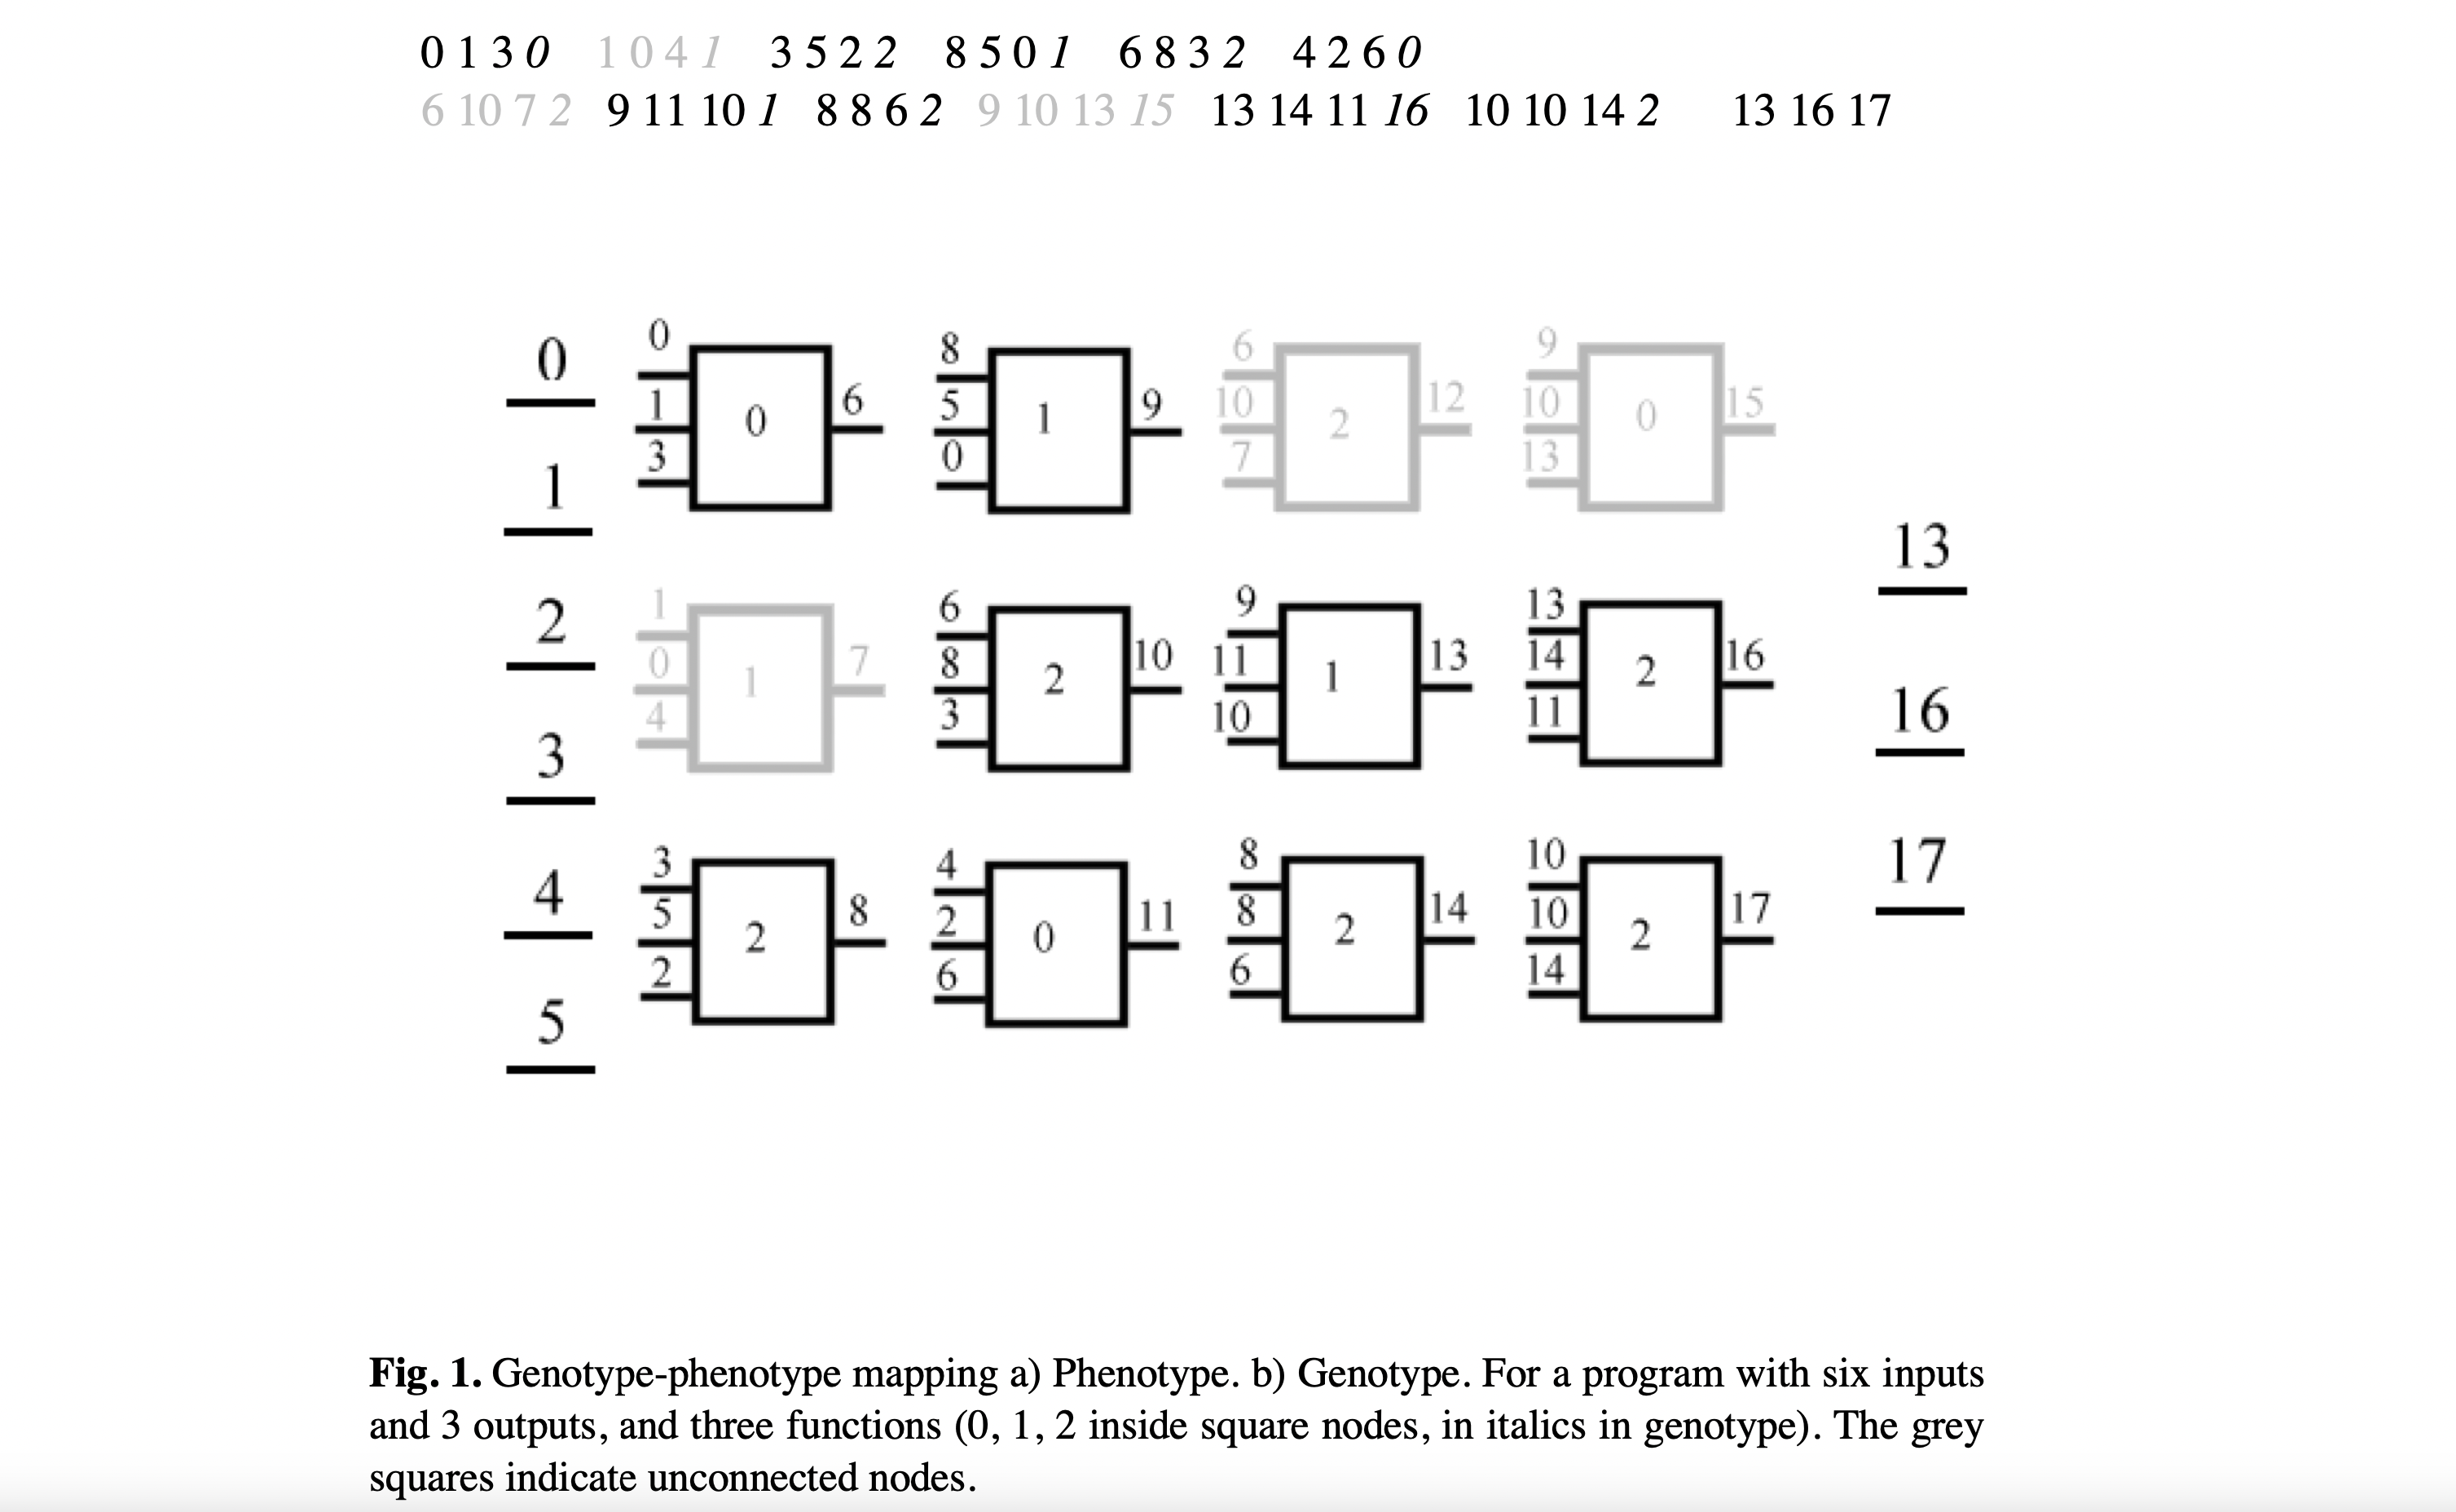
\includegraphics[width=0.65\textwidth]{Screenshot 2025-11-18 at 21.45.10.png}
\caption{Genotype-phenotype mapping for a 3\(\times\)4 CGP grid with levels-back \(l = 2\)}
\label{fig:cgp-mapping}
\end{figure}

\par Every gene \(c_{k,j}\) that addresses the \(k\)-th input of a node in column \(j\) must reference either one of the primary inputs or a node that lies within the previous \(l\) columns. When columns are indexed from zero, this constraint reduces to \(0 \leq c_{k,j} < n_i + j\cdot n_r\) for \(j \leq l\), and \((j-l) n_r \leq c_{k,j} < j n_r\) once the receptive field no longer overlaps with the primary inputs. These inequalities maintain acyclicity automatically and ensure that the decoded phenotypes remain valid directed acyclic graphs.

\par Although modern GP variants embrace Automatically Defined Functions (ADFs), CGP natively provides Automatic Re-used Outputs (AROs) because any node output can be referenced by multiple downstream inputs. Adjusting \(l\) and the grid shape modulates how aggressively reuse is promoted: single-row configurations with \(l = n_c\) maximize reuse opportunities, whereas a single-column grid suppresses them entirely. AROs therefore offer a lightweight alternative to ADFs without introducing additional encoding overhead.

\par In the experiments discussed later in this thesis, two evolutionary strategies were employed for CGP. Symbolic regression benchmarks utilized a generational genetic algorithm with uniform crossover, where each gene of the offspring is sampled independently from its parents. Selection relied on size-two probabilistic tournaments that accept the fitter contestant with probability 0.7, thereby preserving diversity when competing individuals show similar fitness. The Santa Fe Ant Trail variant instead adopted a simple \((1 + \lambda)\) evolutionary strategy with \(\lambda \approx 4\) and mutation-only variation to emphasize local search while retaining a steady-state flavor.

\par The latter strategy proceeds as follows:
\begin{enumerate}
    \item Generate the initial population at random, ensuring that every gene satisfies the CGP constraints.
    \item Evaluate the fitness of all genotypes in the current population.
    \item Promote the best genotype unchanged to the next population (ties are broken randomly among the best-performing candidates).
    \item Populate the remaining \(\lambda\) slots with mutated descendants of the promoted individual.
    \item Repeat steps 2–4 until the termination criterion is met.
\end{enumerate}

\par This workflow highlights how CGP accommodates both crossover-heavy and mutation-centric search schemes while keeping the encoding simple enough to enforce structural validity at every step. The discussion also underscores the close relationship between genotype constraints, reuse mechanisms, and the computational savings targeted in the remainder of the thesis.

\par Figure \ref{fig:fitness-approximation-flow} illustrates the workflow dashboard used to monitor CGP experiments and the adaptive fitness approximation stages that follow each evolutionary update. The screenshot highlights how surrogate-based estimates and full evaluations are interleaved when the stability heuristics indicate that approximation error remains within tolerance.

\begin{figure}[ht]
\centering
\includegraphics[width=0.6\textwidth]{Screenshot 2025-11-25 at 10.01.19.png}
\caption{Workflow view combining CGP evolution and adaptive fitness approximation}
\label{fig:fitness-approximation-flow}
\end{figure}

\section{Fitness Evaluation}
\label{sec:fitness-evaluation}
\par In GP the fitness function acts as the environment that rewards or penalizes whole lineages of candidate programs. Carr emphasizes that this scoring rule is the sole interface between the experimenter’s intent and the stochastic search, so any ambiguity or loophole is inevitably exploited by the evolving population \cite{carr2014}. Designing the metric therefore requires more care than a binary pass/fail test: the function must grade intermediate behaviours so that partially correct individuals can be distinguished from genuinely optimal ones and the search receives meaningful gradients. This idea of awarding “partial credit” steers selection pressure toward the exact behaviours we want and prevents premature convergence on degenerate tricks. Because the fitness evaluator is the only component that directly observes program behaviour, it ultimately determines whether an evolutionary run discovers high-quality solutions or stalls entirely, and—due to repeated execution on every individual—it frequently dominates the overall computational budget.

\section{Problem of High Computational Demand}
\label{sec:high-computational-demand}
Discussion of challenges associated with a large number of evaluations and the need for approximation.

\chapter{Fitness Approximation Methods}
\label{chap:fitness-approximation}

\section{Existing Approaches}
\label{sec:existing-approaches}
Overview of previously published methods for fitness approximation (e.g., model-based, surrogate models, linear regression).

\section{Fitness Inheritance}
\label{sec:fitness-inheritance}
Description of the principle of the Fitness Inheritance method – estimating offspring fitness based on parents.

\section{Key Parameters}
\label{sec:key-parameters}
Proportion of fully evaluated individuals, inheritance coefficient, impact on evolutionary convergence.

\chapter{Proposed Method}
\label{chap:proposed-method}

\section{Mathematical Model and Motivation}
\label{sec:mathematical-model-motivation}
Summary of issues found in existing methods and the rationale for the chosen approach. Formal description of the fitness approximation method, equations, and relationships.

\section{Anticipated Advantages}
\label{sec:anticipated-advantages}
Improved efficiency of evolution, reduced computational load, and impact on result quality.

\chapter{Implementation}
\label{chap:implementation}

\section{Program Architecture and Integration into GP}
\label{sec:architecture-integration}
Implementation description in Python using the \texttt{pandas} and \texttt{matplotlib} libraries. Description of integrating the method into the standard GP cycle (initialization, selection, crossover, mutation, fitness approximation).

\chapter{Experiments}
\label{chap:experiments}

\section{Experimental Setup}
\label{sec:experimental-setup}
Description of datasets, population parameters, and evaluation metrics (time, solution quality, number of evaluations).

\section{Comparison with Reference Version and Results Evaluation}
\label{sec:comparison-results}
Results comparing with classic GP, where all individuals are fully evaluated. Analysis of accuracy, efficiency, and discussion of results.

\chapter{Conclusion}
\label{chap:conclusion}
Summary of achieved results, contributions of the work, and possibilities for future extension.

\begin{thebibliography}{9}

\bibitem{zhou2007}
Zhou, Z., Ong, Y. S., Nair, P. B., Keane, A. J., Lum, K. Y.
\emph{Combining Global and Local Surrogate Models to Accelerate Evolutionary Optimization}.
IEEE Transactions on Systems, Man, and Cybernetics, Part C: Applications and Reviews, 2007.

\bibitem{tzruia2021}
Tzruia, I., Halperin, T., Sipper, M., Elyasaf, A. 
\emph{Fitness Approximation Through Machine Learning with Dynamic Adaptation to the Evolutionary State}. 2021.

\bibitem{starikovGA}
Starikov, A. 
\emph{Genetic Algorithms — Mathematical Apparatus}. Loginom, 2021. 
Available at: \url{https://loginom.ru/blog/ga-math}

\bibitem{drahosova2018}
Drahosova, M., Sekanina, L., Wiglasz, M. 
\emph{Adaptive Fitness Predictors in Coevolutionary Cartesian Genetic Programming}. 2018.

\bibitem{miller2000}
Miller, J. F., Thomson, P. 
\emph{Cartesian Genetic Programming}. 2000.

\bibitem{smith1995}
Smith, R. E., Dike, B. A., Stegmann, S. A. 
\emph{Fitness Inheritance in Genetic Algorithms}. University of Alabama / McDonnell Douglas Corporation, 1995.

\bibitem{bakurov2024}
Bakurov, I., Giuliani, P., Godbey, K., Haut, N., Banzhaf, W., Nazarewicz, W.
\emph{Genetic Programming for the Nuclear Many-Body Problem: a Guide}. 
Facility for Rare Isotope Beams, Michigan State University, 2024.

\bibitem{langdon2008}
Langdon, W. B., Poli, R., McPhee, N. F., Koza, J. R.
\emph{Genetic Programming: An Introduction and Tutorial, with a Survey of Techniques and Applications}.
2008.

\bibitem{carr2014}
Carr, J.
\emph{An Introduction to Genetic Algorithms}.
Whitman College, 2014. Available at: \url{https://www.whitman.edu/Documents/Academics/Mathematics/2014/carrjk.pdf}.

\end{thebibliography}

\appendix
\chapter{Appendices}
\label{chap:appendices}

\section{Example Code for Fitness Inheritance}
\label{sec:example-code}
\begin{lstlisting}[language=Python]
import pandas as pd
import numpy as np

def fitness_inheritance(parent1, parent2, inherit_ratio=0.5):
    """Estimate child fitness based on parents' fitness."""
    return inherit_ratio * parent1 + (1 - inherit_ratio) * parent2

parents = [10, 20]
child_fitness = fitness_inheritance(parents[0], parents[1])
print(child_fitness)
\end{lstlisting}

\section{Additional Materials}
\label{sec:additional-materials}
Graphs, tables, and extended experimental results.

\end{document}
